\section{Resultados}
\label{resultados}
\begin{spacing}{1}

Todo lo comentado en esta sección se ha realizado haciendo uso de la librería linkcomm de R y la ayuda de STRINGdb \cite{HelpNetworks} . 
Tras la obtención de la red de genes al realizar el mapeo con STRINGdb hemos obtenido un grafo como el que podemos observar en la figura \ref{fig:graph1}. En este grafo podemos observar todos los genes que pertenecen a la red asociada al fénomeno de Raynaud. Esto se ha obtenido a partir de STRINGdb como hemos explicado en el apartado \ref{obtencion_red}.

\end{spacing}

\begin{minipage}{\linewidth}
	\makebox[\linewidth]{
		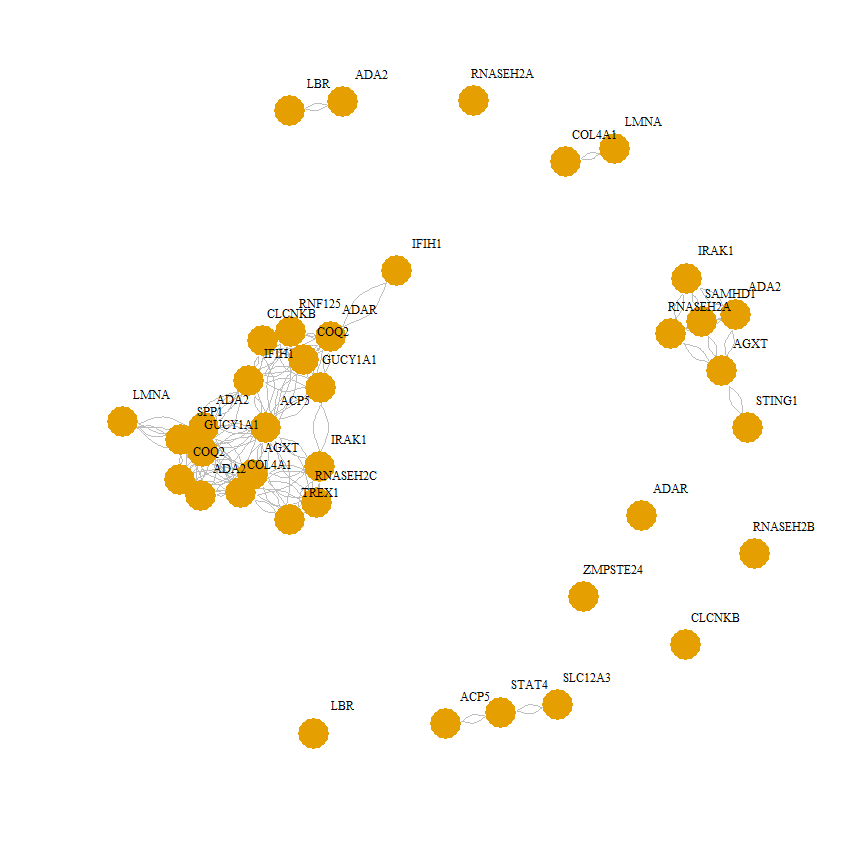
\includegraphics[width=\textwidth]{figures/Raynaud_genes-graph.png}
	}
	\captionof{figure}{Grafo obtenido al realizar el mapeo de genes}
	\label{fig:graph1}
\end{minipage}

\begin{spacing}{1}
	Seguidamente hemos obtenido las comunidades que conforman nuestra red y a las que posteriormente se le harán los estudios de funcionalidad y podremos comprobar que genes conforman el fenotipo más grave de la enfermedad. Se han obtenido 3 gráficas en las que mostramos información acerca de estas comunidades.
	
	En la figura \ref{fig:dendrogram}, la primera obtenida del flujo de trabajo, se observa un dendrograma en la que, diferenciadas por colores, se pueden visualizar las diferentes comunidades obtenidas. Estas se han obtenido a una altura bastante alta (alrededor del 0.9) y nos indica que tenemos 6 comunidades cuyo agrupamiento más grande tiene 11 genes.
\end{spacing}

\begin{minipage}{\linewidth}
	\makebox[\linewidth]{
		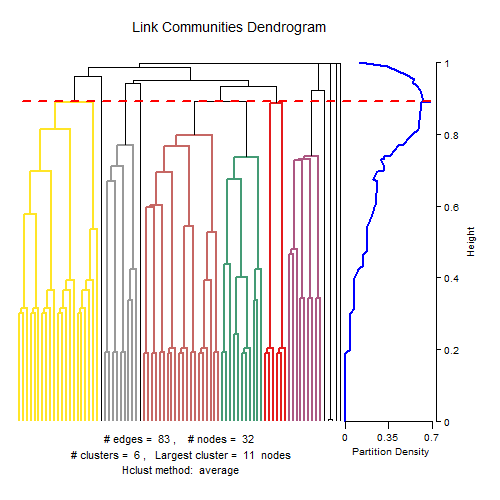
\includegraphics[width=0.7\textwidth]{figures/Raynaud_genes-dendrogram.png}
	}
	\captionof{figure}{Dendrograma de la red mostrando las comunidades}
	\label{fig:dendrogram}
\end{minipage}

\begin{spacing}{1}
La segunda figura que obtenemos del flujo de trabajo sería la número \ref{fig:members}, en esta observamos una matriz de los miembros de cada comunidad. En este caso solo podemos ver los 10 primeros genes de nuestra red y en la matriz se nos muestra las comunidades a las que pertenece cada gen (señalado con un cuadrado en color para cada comunidad a la que pertenece). Además en los márgenes derecho e inferior de la matriz observamos los sumatorios del número de total de comunidades a las que pertenece cada gen y el número de genes que contiene cada comunidad, respectivamente.
\end{spacing}

\begin{minipage}{\linewidth}
	\makebox[\linewidth]{
		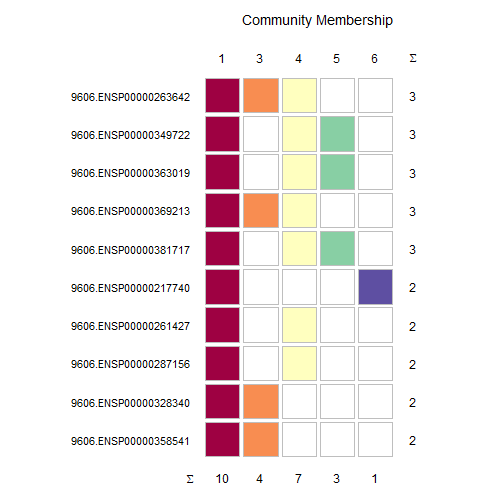
\includegraphics[width=0.7\textwidth]{figures/Raynaud_genes-comunity_members_matrix.png}
	}
	\captionof{figure}{Matriz de los primeros genes para cada comunidad}
	\label{fig:members}
\end{minipage}

\begin{spacing}{1}
	Por último, al obtener las comunidades también hemos mostrado la figura \ref{fig:comunity_graph} en la que se observa un grafo similar al de la figura \ref{fig:graph1}, sin embargo, en este tenemos diferenciadas por colores las diferentes comunidades que hemos obtenido tras realizar el flujo de trabajo.
\end{spacing}

\begin{minipage}{\linewidth}
	\makebox[\linewidth]{
		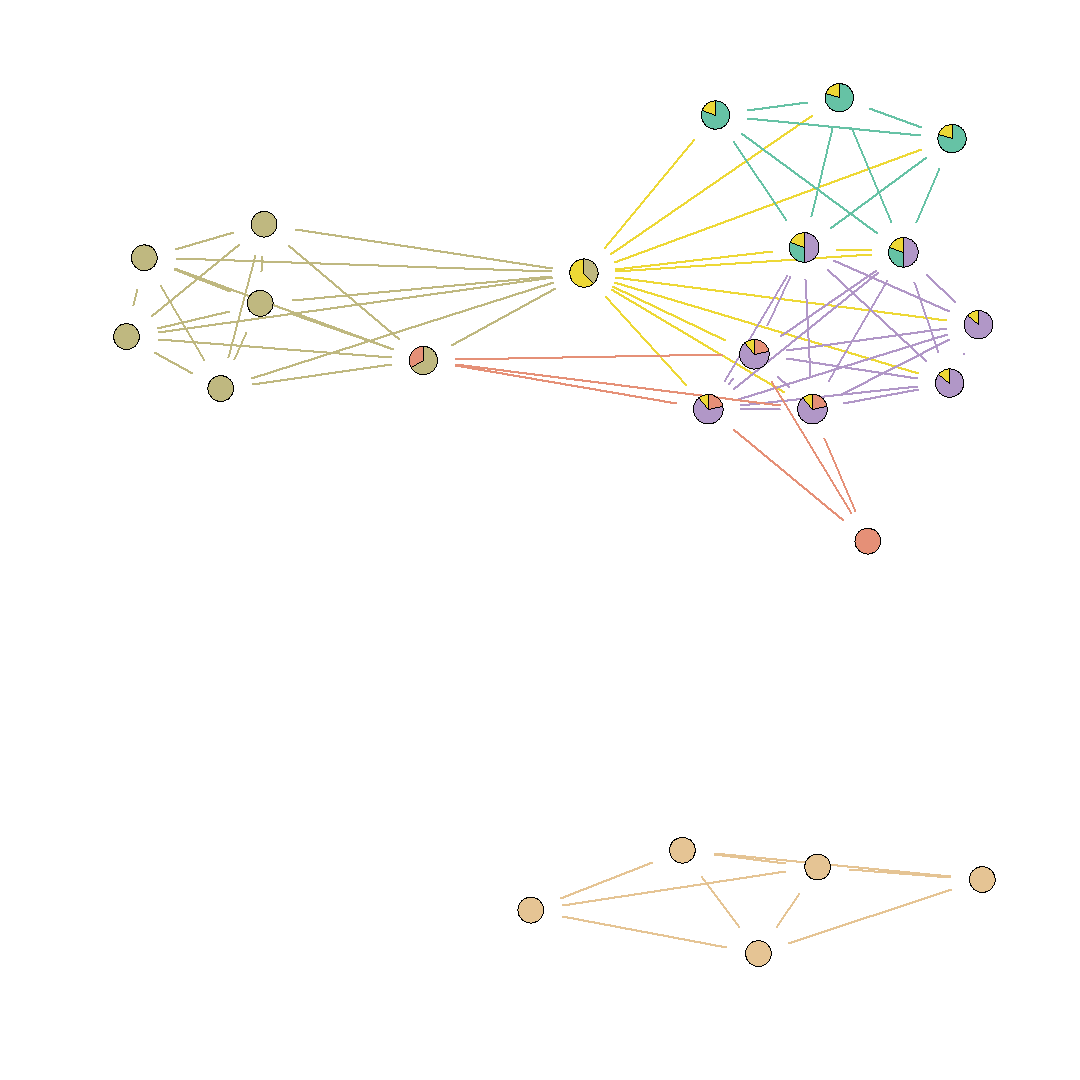
\includegraphics[width=0.7\textwidth]{figures/Raynaud_genes-comunities_graph.png}
	}
	\captionof{figure}{Grafo de los genes divididos por comunidad}
	\label{fig:comunity_graph}
\end{minipage}

\begin{spacing}{1}
Por último, hemos obtenido los CSV de cada una de las comunidades tras aplicarles el enriquecimiento. No todas las comunidades han devuelto una tabla con datos y los datos que sí hemos obtenido podemos observarlos en las tablas \ref{tab:comunity1} y \ref{tab:comunity2}, correspondiendo a las comunidades 1 y 2, respectivamente.

En estas tablas podemos observar las columnas de \textit{Ontología}, que nos indica la ontología de la que se ha obtenido esa referencia; \textit{Término}, que indica el código de la ontología que relaciona a dicho gen; \textit{N genes} y \textit{Genes totales}, que indican el número de genes encontrados y el número de genes que tiene asociado dicho término; en la columna \textit{Genes} vemos los nombres de los genes encontrados; y por último tenemos dos columnas para el \textit{p valor} y el \textit{fdr}, además de una descipción del término de la ontología.
\end{spacing}

\begin{table}[!ht]
	\centering
	\resizebox{\textwidth}{!}{
	\begin{tabular}{|cccccccccc|}
		\hline
		\textbf{Ontología} & \textbf{Categoría} & \textbf{Término} & \textbf{N genes} & \textbf{Genes totales} & \textbf{Taxon Id} & \textbf{genes} & \textbf{p valor} & \textbf{fdr} & \textbf{descripción} \\ \hline
		GO & Process & GO.0032480 & 2 & 43 & 9606 & RNF125,IFIH1 & 5.17e-06 & 0.0011 & negative regulation of type I interferon production \\ 
		GO & Process & GO.0045088 & 2 & 361 & 9606 & RNF125,IFIH1 & 0.00034 & 0.018 & regulation of innate immune response \\ 
		GO & Process & GO.0043900 & 2 & 653 & 9606 & RNF125,IFIH1 & 0.0011 & 0.0347 & regulation of multi-organism process \\ 
		GO & Process & GO.0032446 & 2 & 690 & 9606 & RNF125,IFIH1 & 0.0012 & 0.0347 & protein modification by small protein conjugation \\ \hline
	\end{tabular}
	}
	\vspace{5px}
	\caption{Resultado del enriquecimiento de la comunidad 1}
	\label{tab:comunity1}
\end{table}

\begin{table}[!ht]
	\centering
	\resizebox{\textwidth}{!}{
	\begin{tabular}{|c|ccccccccc|}
		\hline
		\textbf{Ontología} & \textbf{Categoría} & \textbf{Término} & \textbf{N genes} & \textbf{Genes totales} & \textbf{Taxon Id} & \textbf{genes} & \textbf{p valor} & \textbf{fdr} & \textbf{descripción} \\ \hline
		GO & Process & GO.0090305 & 4 & 287 & 9606 & RNASEH2A,SAMHD1,TREX1,RNASEH2B & 2.37e-07 & 4.26e-05 & nucleic acid phosphodiester bond hydrolysis \\ 
		GO & Process & GO.0034655 & 4 & 394 & 9606 & RNASEH2A,SAMHD1,RNASEH2C,RNASEH2B & 8.29e-07 & 7.46e-05 & nucleobase-containing compound catabolic process \\ 
		GO & Process & GO.0090501 & 3 & 137 & 9606 & RNASEH2A,SAMHD1,RNASEH2B & 3.55e-06 & 9.12e-05 & RNA phosphodiester bond hydrolysis \\ 
		GO & Process & GO.0006401 & 3 & 237 & 9606 & RNASEH2A,RNASEH2C,RNASEH2B & 1.79e-05 & 4e-04 & RNA catabolic process \\ 
		GO & Process & GO.0006298 & 2 & 26 & 9606 & RNASEH2A,TREX1 & 1.97e-05 & 4e-04 & mismatch repair \\ 
		GO & Process & GO.0090502 & 2 & 70 & 9606 & RNASEH2A,RNASEH2B & 0.00013 & 0.0024 & RNA phosphodiester bond hydrolysis, endonucleolytic \\ 
		GO & Process & GO.0090304 & 5 & 3941 & 9606 & RNASEH2A,SAMHD1,TREX1,RNASEH2C,RNASEH2B & 0.00033 & 0.0046 & nucleic acid metabolic process \\ 
		GO & Process & GO.0006260 & 2 & 203 & 9606 & RNASEH2A,TREX1 & 0.0011 & 0.01 & DNA replication \\ 
		GO & Process & GO.0016070 & 4 & 3430 & 9606 & RNASEH2A,SAMHD1,RNASEH2C,RNASEH2B & 0.0041 & 0.0318 & RNA metabolic process \\ \hline
	\end{tabular}
	}
	\vspace{5px}
	\caption{Resultado del enriquecimiento de la comunidad 2}
	\label{tab:comunity2}
\end{table}